\chapter{Results}\label{results}

To present our results we would like to refer to two videos created as part of the assignment. The first \ref{fig:franka-sim} was done in the Gazebo environment and it performs smoothly and in expected manner. The same could be seen in the video made in the real life setting \ref{fig:franka-real} by applying the same trajectory generators. 


\begin{figure}[htpb]
    \centering
    \includegraphics[width=0.45\textwidth]{figures/franka-sim.png}
    \caption{\href{https://gitlab.lrz.de/tum-impl-ss24/assignment2-group1/-/blob/main/media/content/gazebo-whiteboard-task-simulation.mov}{Simulation video (lrz link)}}
    \label{fig:franka-sim}
\end{figure}
\begin{figure}[htpb]
    \centering
    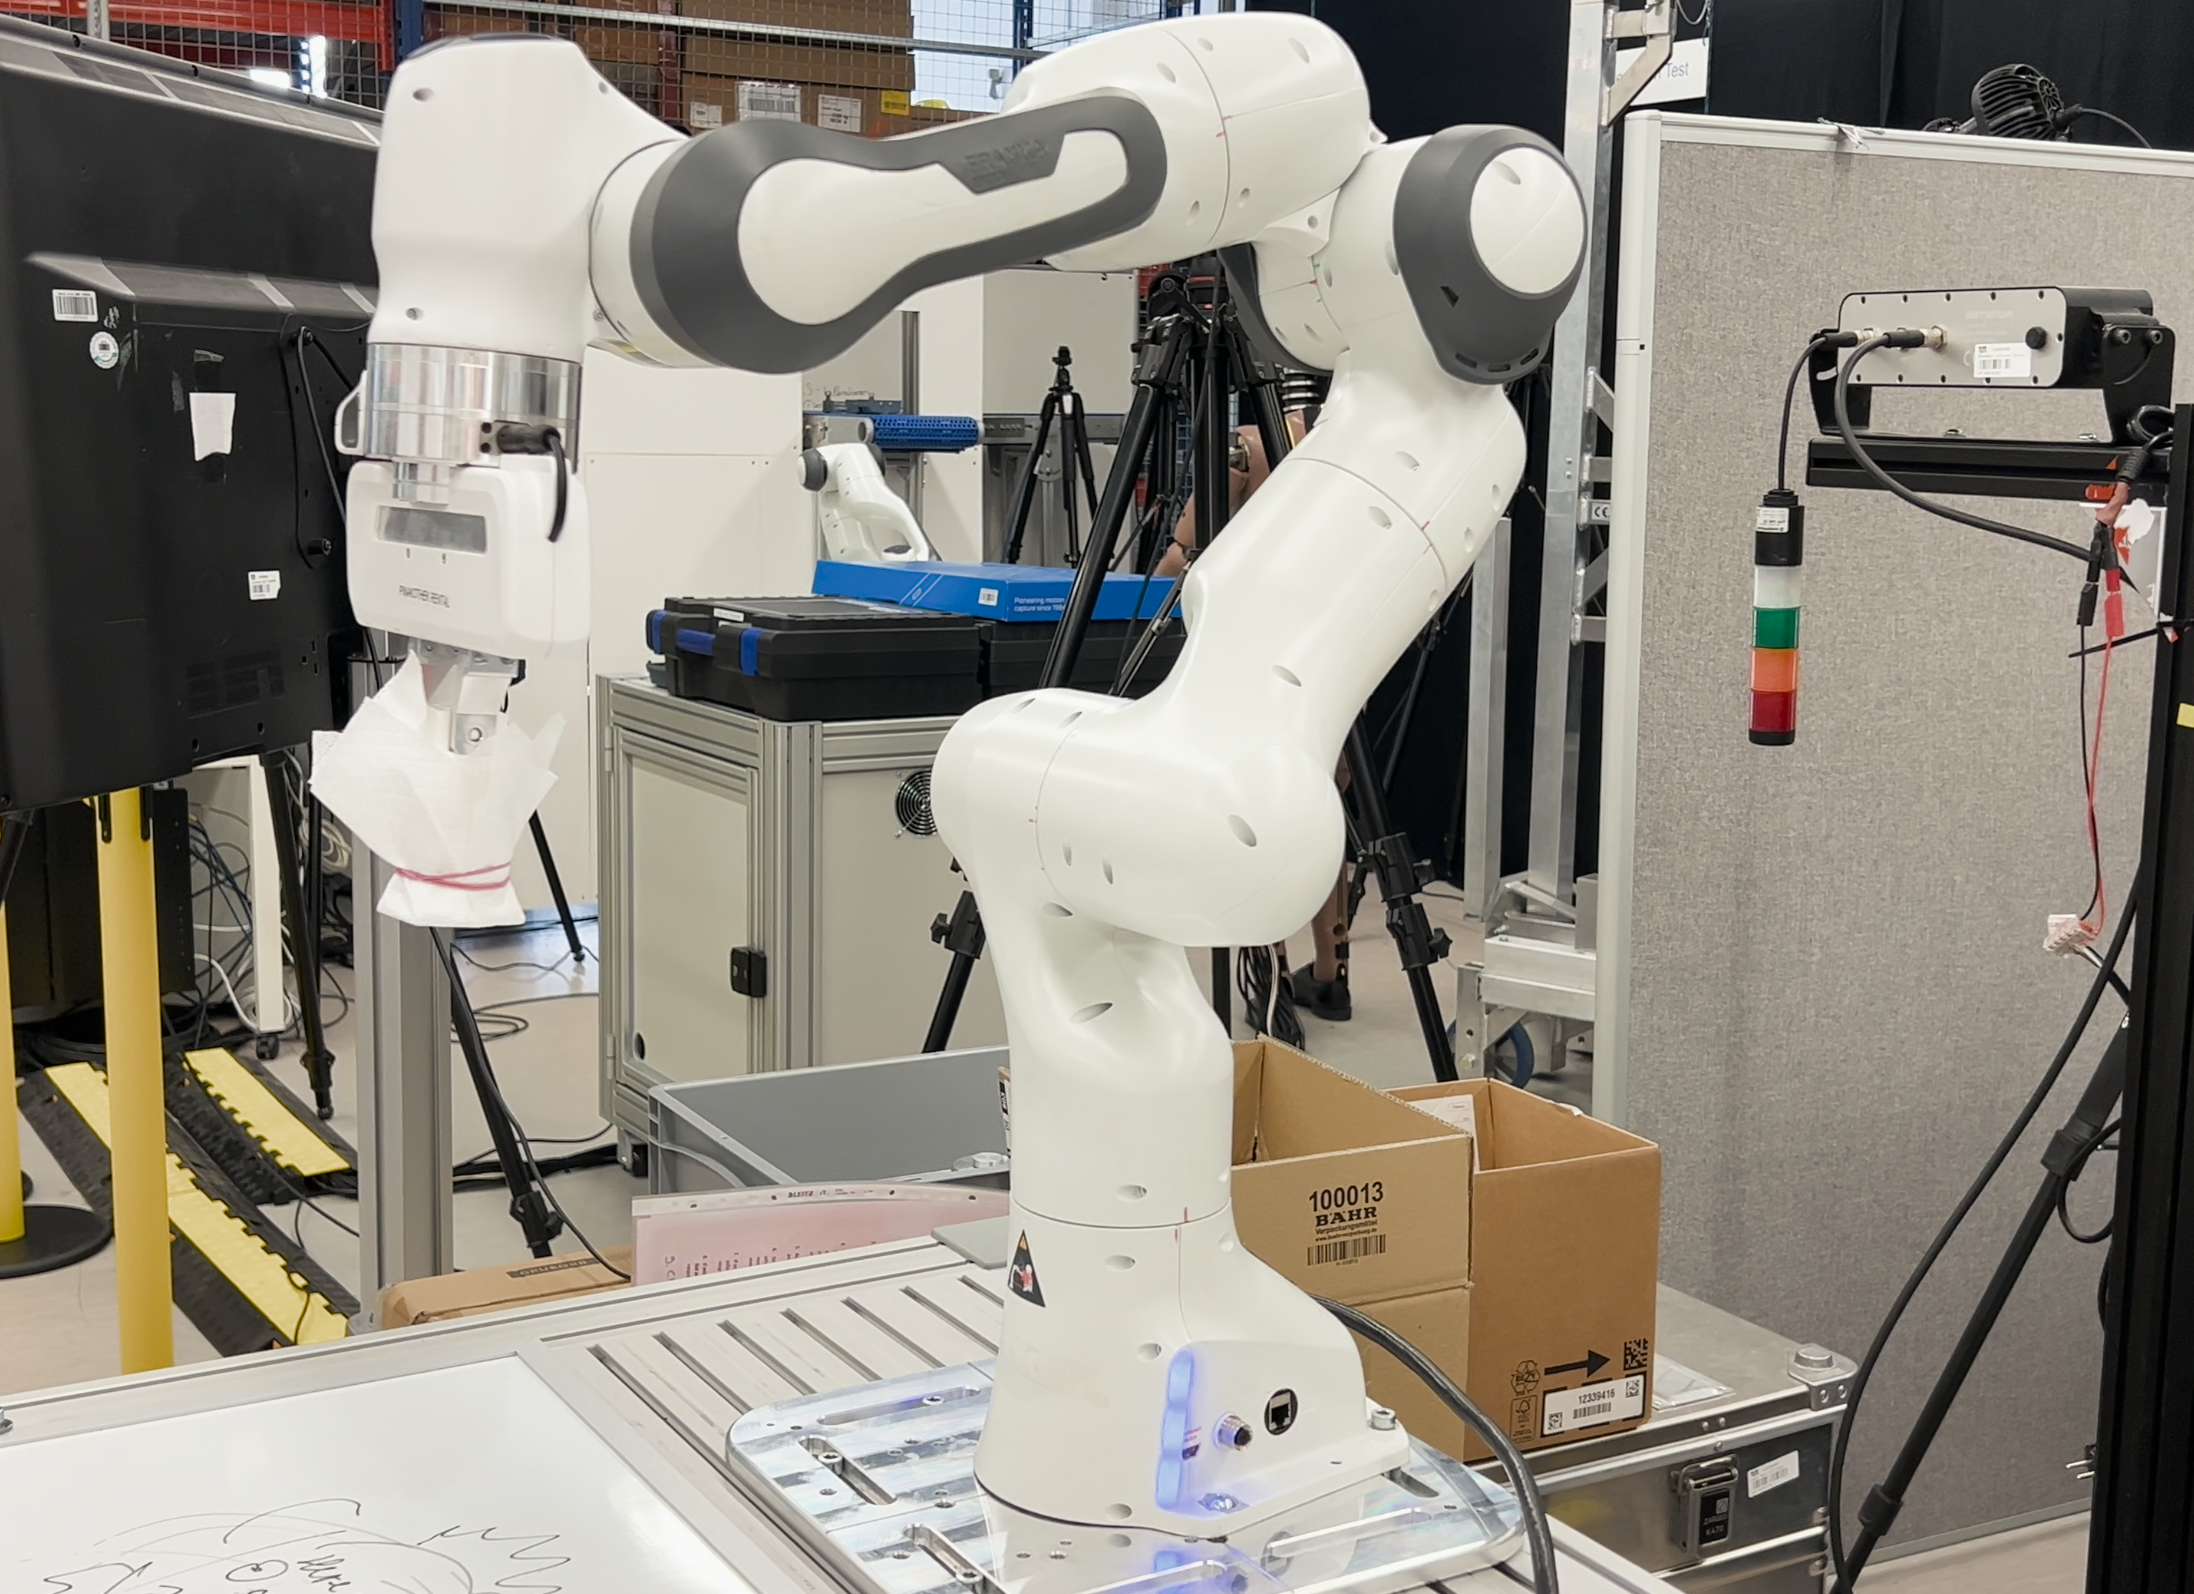
\includegraphics[width=0.45\textwidth]{figures/random-franka.png}
    \caption{\href{https://gitlab.lrz.de/tum-impl-ss24/assignment2-group1/-/raw/main/media/content/cleaning-whiteboard-task.mp4}{Linear movement towards the surface}}
    \label{fig:franka-real}
\end{figure}


Moreover, we have also conducted several experiments which involved changing impedance controller stiffness. It is interesting to notice how stiffness changes sensitivity of the controller.

\clearpage
\begin{figure}[htb]
    \centering
    \begin{subfigure}{0.46\textwidth}
        \centering
        \includegraphics[width=\textwidth, height=0.3\textheight]{figures/p10.png}
        \caption{Position with linear stiffness = 10 }
        \label{fig:franka-pos-10-bag}
    \end{subfigure}
    \hfill
    \begin{subfigure}{0.46\textwidth}
        \centering
        \includegraphics[width=\textwidth, height=0.3\textheight]{figures/p13.png}
        \caption{Position with linear stiffness = 13}
        \label{fig:franka-pos-13-bag}
    \end{subfigure}

    \caption{Position (x,y,z) changes through time}
    \label{fig:franka-pos-bag}
\end{figure}

From the position change graph we can conclude that controller behaves little better with bigger stiffness, however, does not provide that much of the difference for the z coordinate which we are most interested in.


\begin{figure}[htbp]
    \centering
    \begin{subfigure}{0.46\textwidth}
        \centering
        \includegraphics[width=\textwidth, height=0.3\textheight]{figures/f10.png}
        \caption{Force change with linear stiffness = 10 }
        \label{fig:franka-f-10-bag}
    \end{subfigure}
    \hfill
    \begin{subfigure}{0.46\textwidth}
        \centering
        \includegraphics[width=\textwidth, height=0.3\textheight]{figures/f13.png}
        \caption{Force change with linear stiffness = 13}
        \label{fig:franka-f-13-bag}
    \end{subfigure}

    \caption{Force changes through time}
    \label{fig:franka-pos-bag}
\end{figure}

We can see the same relation in the force change graph. One last important thing is to notice how position change forms a trapezoid form, exactly as we have programmed it to do.


 